%%%%%%%%%%%%%%%%%%%%%%%%%%%%%%%%%%%%%%%%
%% MCM/ICM LaTeX Template %%
%% 2024 MCM/ICM           %%
%%%%%%%%%%%%%%%%%%%%%%%%%%%%%%%%%%%%%%%%
\documentclass[12pt]{article}
\usepackage{geometry}
\geometry{a4paper, margin=1in}
\usepackage{setspace}
\usepackage{listings}
\usepackage{booktabs}
\usepackage{xcolor}
\usepackage{caption}
\usepackage{amsmath}
\usepackage{fancyhdr}
\usepackage{graphicx}
\usepackage{setspace}
\usepackage{float}
\usepackage{wrapfig}
\usepackage{ctex}
\usepackage{subcaption}
\usepackage{color}
\usepackage{listings}
\usepackage{array}
\usepackage{booktabs}
\usepackage{enumitem}
\usepackage{hyperref} % 包含超链接包
\lstset{ %
language=C++,
basicstyle=\footnotesize,
numbers=left,
numberstyle=\footnotesize,
stepnumber=1,
numbersep=5pt,
backgroundcolor=\color{white},
showspaces=false,
showstringspaces=false,
showtabs=false,
frame=single,
tabsize=2,
captionpos=b,
breaklines=true,
breakatwhitespace=false,
escapeinside={(*@}{@*)}
}
\usepackage[colorlinks,linkcolor=blue]{hyperref}
\lstdefinestyle{mystyle}{
    backgroundcolor=\color{white},   % 背景色
    commentstyle=\color{green},      % 注释颜色
    keywordstyle=\color{blue},       % 关键词颜色
    numberstyle=\tiny\color{gray},   % 行号样式
    basicstyle=\small\ttfamily,      % 基本样式
    breakatwhitespace=false,         % 是否在空白字符断行
    breaklines=true,                 % 是否自动断行
    captionpos=b,                   % 标题位置(b底部,t顶部)
    keepspaces=true,                 % 保留空格
    numbers=left,                    % 行号位置
    numbersep=5pt,                   % 行号与代码的距离
    showspaces=false,                % 是否显示空格
    showstringspaces=false,          % 是否显示字符串中的空格
    showtabs=false,                  % 是否显示制表符
    tabsize=4                        % 制表符大小
}
\lstset{style=mystyle}
\geometry{left=1in,right=0.75in,top=1in,bottom=1in}

%%%%%%%%%%%%%%%%%%%%%%%%%%%%%%%%%%%%%%%%
% Replace ABCDEF in the next line with your chosen problem
% and replace 1111111 with your Team Control Number
%%%%%%%%%%%%%%%%%%%%%%%%%%%%%%%%%%%%%%%%

\usepackage{newtxtext}
\usepackage{indentfirst} 
\usepackage{enumitem}
\usepackage{amsmath,amssymb,amsthm}
\usepackage{newtxmath} % must come after amsXXX
\usepackage{xcolor}
\usepackage{graphicx}

\usepackage{fancyhdr}
\rhead{}
\cfoot{}
\pagestyle{fancy}
\newtheorem{theorem}{Theorem}
\newtheorem{corollary}[theorem]{Corollary}
\newtheorem{lemma}[theorem]{Lemma}
\newtheorem{definition}{Definition}
\setlength{\parindent}{2em} % 设置首行缩进为2em
\usepackage{hyperref}
\hypersetup{
    colorlinks=true,
    linkcolor=black,  % 调整链接颜色为黑色,包括引用标记
    citecolor=black,  % 调整引用文献颜色为黑色
    filecolor=magenta,
    urlcolor=cyan
}
\begin{document}
\graphicspath{{.}}  % Place your graphic files in the same directory as your main document
\DeclareGraphicsExtensions{.pdf, .jpg, .tif, .png}
\thispagestyle{empty}
\vspace*{-16ex}
% to here
%%%%%%%%%%% End Summary %%%%%%%%%%%
%%%%%%%%%%%%%%%%%%%%%%%%%%%%%%
\pagestyle{fancy}
% Uncomment the next line to generate a Table of Contents
\tableofcontents
\newpage
\setcounter{page}{2}
\rhead{Page \thepage\  of \pageref{LastPage}}
%%%%%%%%%%%%%%%%%%%%%%%%%%%%%%
\section{文本情感分析概述}
文本情感分析是自然语言处理(NLP)领域中的一项重要技术,主要目的是从文本数据中识别和提取情感倾向。这项技术广泛应用于社交媒体监控、品牌声誉管理、市场研究、客户服务等多个领域。通过情感分析,企业和组织能够理解公众情感,优化产品和服务,同时更好地与用户进行互动。
\subsection{情感分析的类型}
情感分析主要可以分为三类:二分类、多分类和情感倾向性分析。二分类是最简单的类型,通常将情感分为正面和负面两种。多分类则在此基础上进一步细分,例如将情感划分为非常正面、正面、中性、负面和非常负面等。情感倾向性分析则尝试从文本中提取更具体的情感状态,如愤怒、快乐、悲伤等。
\subsection{情感分析的技术方法}
情感分析的技术方法主要分为基于词典的方法和基于机器学习的方法。基于词典的方法依赖于预定义的情感词典,通过匹配文本中的词汇与词典中的条目来确定文本的情感倾向。这种方法简单直观,但灵活性和准确性受限于词典的质量和覆盖范围。

基于机器学习的方法则是当前最流行的技术,特别是随着深度学习技术的发展,基于神经网络的模型如CNN(卷积神经网络)和RNN(递归神经网络)的变体,例如LSTM(长短期记忆网络)和BiLSTM(双向长短期记忆网络),在情感分析领域表现出了优异的性能。这些模型能够通过学习大量的文本数据,捕捉语言的复杂特征,从而更准确地预测文本的情感倾向。
\subsection{中文情感分析的挑战}
与英文相比,中文情感分析面临额外的挑战,主要来源于中文的语言特性,如语法结构的复杂性和词语的多义性。此外,中文文本中的表情符号和网络用语的广泛使用也给情感分析带来了新的挑战。因此,开发适用于中文的高效算法是当前研究的热点之一。

在此基础上,本研究通过结合CNN和BiLSTM模型,对中文文本进行情感分析,旨在利用CNN的强大特征提取能力和BiLSTM的序列数据处理能力,提高情感分类的准确性和效率。

\section{成员与分工}
\begin{table}[H]
    \centering
    \begin{tabular}{c@{\hspace{30pt}}c@{\hspace{30pt}}c}
        \toprule
        学号 & 姓名 & 分工 \\
        \midrule
        21009200817& 杨铠铭& 编程实现,代码调试,报告撰写\\
        21009200051& 卢羿& 编程实现,代码调试,报告撰写 \\
        21049200133& 孙博& 编程实现,代码调试,报告撰写 \\
        \bottomrule
    \end{tabular}
    \caption{成员信息表}
    \label{tab:example}
\end{table}

\section{模型架构与方法}
\subsection{数据准备}
\subsubsection{语料准备}

语料的选择为谭松波老师的评论语料\cite{hotel-comment},正负例各2000。属于较小的数据集,本项目包含了原始语料。将原本gb2312编码文件转换成utf-8编码的文件。

\subsubsection{词向量准备}

本实验使用开源词向量chinese-word-vectors\cite{P18-2023},选择知乎语料训练而成的Word Vector。

\subsection{基于CNN实现}
\subsubsection{CNN基本结构}
卷积神经网络(Convolutional Neural Network, CNN)是一种深度学习模型,特别擅长处理具有网格拓扑结构的数据。CNN 由多个层(layers)组成,每一层执行特定的功能。主要包括以下几种层:
\begin{enumerate}
    \item \textbf{输入层(Input Layer)}\newline
    通常是一个三维数组(高度 × 宽度 × 通道)
    \item \textbf{卷积层(Convolutional Layer)}
    \begin{itemize}
        \item 通过卷积核(filters)对输入进行卷积操作,提取局部特征。每个卷积核在输入图像上滑动,执行点积运算,生成特征图(feature map)
        \item 卷积操作公式:
        \begin{equation}
            (I \ast K)(x, y) = \sum_m \sum_n I(m, n) \cdot K(x - m, y - n)
        \end{equation}
        其中,\( I \) 是输入,\( K \) 是卷积核,\((x, y)\) 是输出特征图的位置
        \item 填充(Padding)
        \begin{itemize}
            \item Valid Padding: 不使用填充,卷积会导致输出尺寸减小
            \item Same Padding: 使用填充,使输出尺寸与输入相同
        \end{itemize}
        \item 步幅(Stride)\newline
        卷积核在输入图像上滑动的步长。步幅越大,输出特征图尺寸越小。
    \end{itemize}
    \item \textbf{激活层(Activation Layer)}
    \begin{itemize}
        \item 通常使用 ReLU(Rectified Linear Unit)激活函数,将非线性引入模型
        \item 公式:
        \begin{equation}
            f(x) = \max(0, x)
        \end{equation}
        其他常见的激活函数包括 Sigmoid、Tanh 等
    \end{itemize}
    \item \textbf{池化层(Pooling Layer)}\newline
    池化层通过下采样操作(如最大池化或平均池化)减少特征图的尺寸,降低计算量和参数量,同时保留重要特征。
    \begin{itemize}
        \item 最大池化公式:
        \begin{equation}
            y = \max(x_i)
        \end{equation}
        \item 平均池化公式:
        \begin{equation}
            y = \frac{1}{n} \sum_{i=1}^{n} x_i
        \end{equation}
    \end{itemize}
    \item \textbf{全连接层(Fully Connected Layer)}\newline
    全连接层将前一层的特征展平成一维向量,与权重矩阵相乘并加上偏置,进行分类或回归任务。\newline
    全连接层公式:
    \begin{equation}
        y = Wx + b
    \end{equation}
    \item \textbf{输出层(Output Layer)}\newline
    输出层根据任务的不同可以使用不同的激活函数。例如,softmax 激活函数用于多分类任务,sigmoid 用于二分类任务。
\end{enumerate}
\subsubsection{基于CNN的中文情感分析模型}

根据Zhang, Ye等人\cite{zhang2015sensitivity}的关于CNN的情感分析的研究和相关博客\cite{CNN-text-classification-tf},实现了我们的基于CNN的中文情感分析模型。模型的架构如图\ref{fig:CNN}所示。

首先,我们采用了基于预训练词向量的单通道,将语料进行Embedding后,输入给带有多层滤波器和特征如的卷积神经网络。这里我们实现了多个不同长度的定宽卷积核。

随后,将CNN网络的输出传给最大池化层,对每个滤波器的输出仅取一个最大值。

最后,输入给带有Dropout和Softmax的全连接层,得到最终模型输出。经过Softmax操作,我们得到了对输入语句的情感分析结果(积极-POS,消极-NEG)的概率。

对于模型实现的细节,我们在代码实现部分进行了详细分析。

\begin{figure}[H]
    \centering
    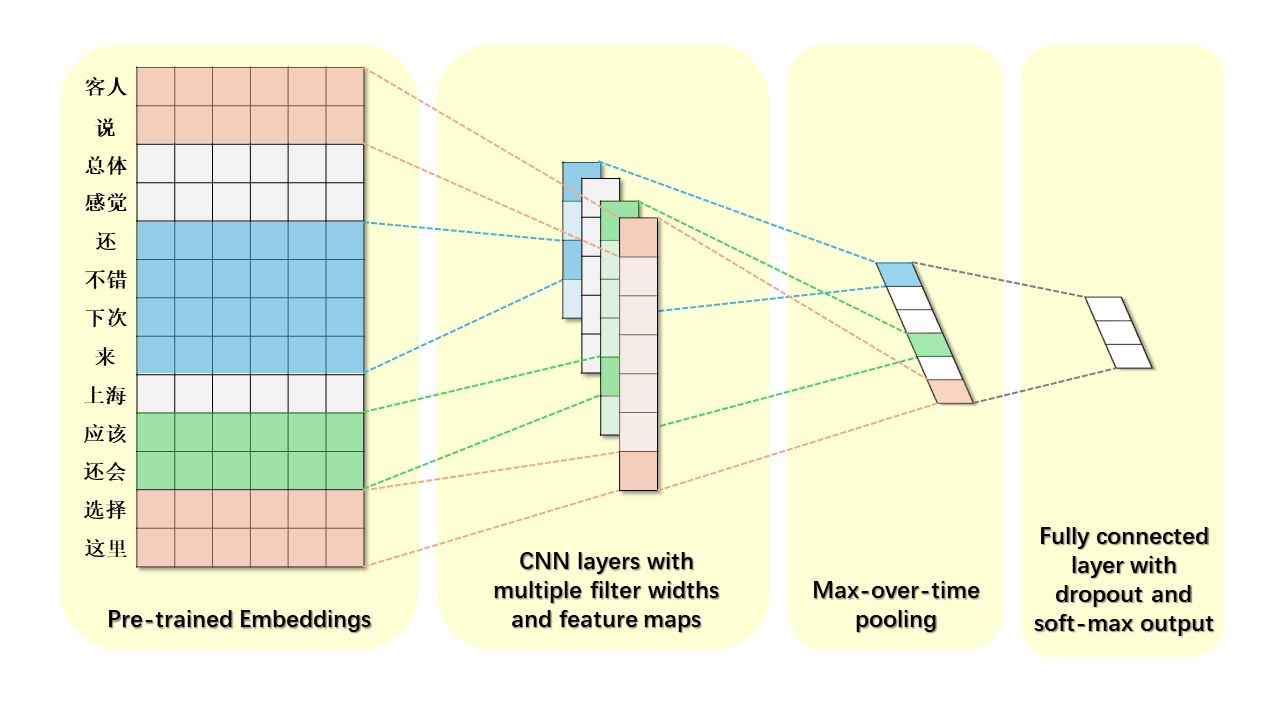
\includegraphics[width=1.0\linewidth]{sections//fig/cnn.png}
    \caption{基于CNN的中文情感分析}
    \label{fig:CNN}
\end{figure}

\subsection{基于BiLSTM实现}
\subsubsection{BiLSTM基本结构}
双向长短期记忆网络(Bidirectional Long Short-Term Memory,BiLSTM)是一种用于处理序列数据的深度学习模型,广泛应用于自然语言处理任务中,如情感分析、机器翻译和语音识别等。
\begin{enumerate}
    \item \textbf{LSTM单元}\newline
    LSTM单元是BiLSTM的基本构建模块。标准的RNN容易在处理长序列时遗忘前面的信息,而LSTM通过引入记忆单元(Cell State)和三个门控机制(输入门、遗忘门、输出门)来有效缓解这一问题。LSTM单元在每个时间步的计算如下:
    \begin{itemize}
        \item \textbf{遗忘门(Forget Gate):}决定需要遗忘的上一个时间步的信息。计算公式如下:\newline
        \begin{equation}
            f_t = \sigma(W_f \cdot [h_{t-1}, x_t] + b_f)
        \end{equation}
        其中,$\sigma$ 是Sigmoid激活函数,$W_f$ 是权重矩阵,$h_{t-1}$ 是上一个时间步的隐藏状态,$x_t$ 是当前时间步的输入,$b_f$ 是偏置项。
        \item \textbf{输入门(Input Gate):}决定新的信息要更新到记忆单元中的哪些部分。计算公式如下:
        \begin{equation}
            i_t = \sigma(W_i \cdot [h_{t-1}, x_t] + b_i)
        \end{equation}
        \begin{equation}
            \tilde{C}_t = \tanh(W_C \cdot [h_{t-1}, x_t] + b_C)
        \end{equation}
其中,$\tanh$ 是双曲正切激活函数,$W_i$ 和 $W_C$ 是权重矩阵,$b_i$ 和 $b_C$ 是偏置项,$\tilde{C}_t$ 是新的候选记忆单元状态。
        \item \textbf{记忆单元更新:}结合遗忘门和输入门的信息,更新记忆单元状态。计算公式如下:
        \begin{equation}
            C_t = f_t \cdot C_{t-1} + i_t \cdot \tilde{C}_t
        \end{equation}
        \item \textbf{输出门(Output Gate):}决定隐藏状态的输出。计算公式如下:
        \begin{equation}
            o_t = \sigma(W_o \cdot [h_{t-1}, x_t] + b_o)
        \end{equation}
        \begin{equation}
            h_t = o_t \cdot \tanh(C_t)
        \end{equation}
    \end{itemize}
    在这些公式中,$C_t$ 是记忆单元的状态,$h_t$ 是隐藏状态。
    \item \textbf{双向机制}\newline
    BiLSTM通过结合正向和反向的LSTM层,进一步增强模型对上下文信息的捕捉能力。
    \begin{itemize}
        \item \textbf{正向LSTM:}从序列的前向后处理数据,生成正向隐藏状态序列 $\overrightarrow{h_t}$:
        \begin{equation}
            \overrightarrow{h_t} = \text{LSTM}(x_t, \overrightarrow{h_{t-1}}, \overrightarrow{C_{t-1}})
        \end{equation}
        \item \textbf{反向LSTM:}从序列的后向前处理数据,生成反向隐藏状态序列 $\overleftarrow{h_t}$:
        \begin{equation}
            \overleftarrow{h_t} = \text{LSTM}(x_t, \overleftarrow{h_{t+1}}, \overleftarrow{C_{t+1}})
        \end{equation}
    \end{itemize}
    在每个时间步t,正向隐藏状态和反向隐藏状态会被连接起来,形成最终的隐藏状态 $h_t$:
    \begin{equation}
        h_t = [\overrightarrow{h_t}; \overleftarrow{h_t}]
    \end{equation}

\end{enumerate}
\subsubsection{基于BiLSTM的中文情感分析模型}

BiLSTM在自然语言处理领域展示着优越的性能\cite{huang2015bidirectional}。ELMo\cite{sarzynska2021detecting}使用了BiLSTM作为模型的基础,展示了在情感分析和其他 NLP 任务上的卓越表现。不难发现,BiLSTM通过捕捉全面的上下文信息、处理长距离依赖关系、适应多样化的句子结构以及对抗文本噪声等优势,使其在情感分析任务中表现优异。所以,我们尝试使用BiLSTM模型处理中文情感分析。

基于BI-LSTM模型的中文情感分析模型有如下步骤:

\begin{itemize}[noitemsep, topsep=1pt, partopsep=1pt, parsep=1pt, left=32pt]
    \item 中文词嵌入层。
    \item 使用BI-LSTM模型。
    \item 带有Softmax的全连接。
\end{itemize}

\vspace{8pt}

基于BiLSTM的中文情感分析的模型架构如图\ref{fig:bilstm}所示。

\vspace{8pt}

\begin{figure}[H]
    \centering
    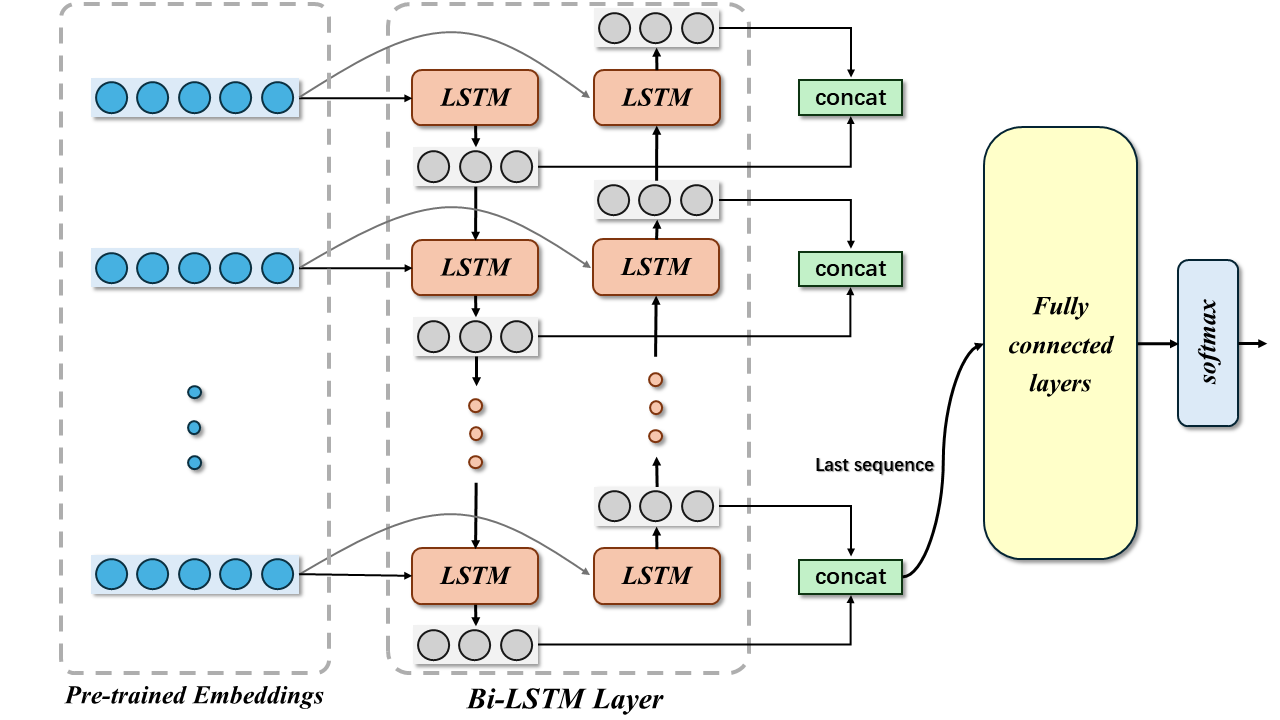
\includegraphics[width=1.0\linewidth]{sections//fig/bilstm.png}
    \caption{基于BI-LSTM的中文情感分析}
    \label{fig:bilstm}
\end{figure}

对于模型实现的细节,我们在代码实现部分进行了详细分析。
\section{代码实现}

\subsection{基于CNN的中文情感分析}
以下是代码实现的主要文件及设计思路描述:

\begin{itemize}
    \item main.py: 包含了数据处理、模型构建和训练的逻辑。从数据源加载并预处理数据,使用jieba进行中文分词,生成适合模型训练的数据格式。定义了输入函数(input\_fn)和模型函数(model\_fn),构建了一个基于CNN的文本分类模型。使用AdamOptimizer进行模型训练,并计算损失函数和评估指标。
    \item export.py: 通过Estimator.export\_saved\_model将训练好的模型导出,以便后续部署使用。
    \item serve.py: 加载导出的模型,并提供预测服务功能。
    \item debug.py: 用于调试数据输入和模型调用,方便开发时的调试工作。启用了eager\_execution,可以逐步执行代码并查看各个步骤的输出结果。
\end{itemize}

下面仅对main.py中的基于CNN的模型训练部分的核心内容进行分析:

\subsubsection{检查features类型}

    \begin{lstlisting}
if isinstance(features, dict): 
    features = features['words']\end{lstlisting}

如果是字典,则从中提取键为'words'的值,将其赋给features。这种结构的设计可能是为了支持不同类型的输入数据。

\subsubsection{定义词嵌入层}

    \begin{lstlisting}
# Word Embedding
embedding_size = 100
embeddings = tf.get_variable('embedding', [vocab_size, embedding_size])
embed = tf.nn.embedding_lookup(embeddings, input_x)
embed_expanded = tf.expand_dims(embed, -1)\end{lstlisting}
\begin{itemize}
    \item embedding\_size表示嵌入向量的维度。
    \item tf.get\_variable用来获取或创建名为'embedding'的变量,其形状为[vocab\_size, embedding\_size],表示单词表大小为vocab\_size,每个单词的嵌入向量embedding\_size维。
    \item tf.nn.embedding\_lookup将输入的词汇索引input\_x查找并获取对应的嵌入向量。
    \item tf.expand\_dims(embed, -1)在最后一个维度(-1表示最后一个维度)上增加一个维度,用于后续卷积操作。
\end{itemize}

\subsubsection{定义卷积神经网络}

首先定义卷积和池化层:

\begin{lstlisting}
pooled_outputs = []
for i, filter_size in enumerate(params['filter_sizes']):
    conv2 = tf.layers.conv2d(embeddings_expanded, params['num_filters'], kernel_size=[filter_size, params['dim']],
                             activation=tf.nn.relu, name='conv-{}'.format(i))
    pooled = tf.layers.max_pooling2d(inputs=conv2, pool_size=[params['nwords'] - filter_size + 1, 1],
                                     strides=[1, 1], name='pool-{}'.format(i))
    pooled_outputs.append(pooled)\end{lstlisting}

\begin{itemize}
    \item 卷积层 (conv2d):在循环中,对每个指定大小的卷积核 (filter\_size),使用 tf.layers.conv2d 创建一个卷积层。这一层会对输入图像或特征图进行卷积操作,并使用 ReLU 激活函数。
    \item 池化层 (max\_pooling2d):紧接着卷积层,应用最大池化操作。这里的池化窗口大小是 $[params['nwords'] - filter_size + 1, 1]$,指定了在空间维度上的窗口大小和步幅。最大池化有助于提取特征并减少维度。
    \item     每个卷积核大小对应的卷积层和池化层结果都被添加到 pooled\_outputs 列表中。
\end{itemize}

\subsubsection{定义全连接层和输出}

\begin{lstlisting}
num_total_filters = params['num_filters'] * len(params['filter_sizes'])
h_pool = tf.concat(pooled_outputs, 3)
output = tf.reshape(h_pool, [-1, num_total_filters])
output = tf.layers.dropout(output, rate=dropout, training=training)
logits = tf.layers.dense(output, num_tags)
pred_ids = tf.argmax(input=logits, axis=1)\end{lstlisting}

\begin{itemize}
    \item 计算出所有卷积核的总数后,将所有池化层的结果在深度维度上连接成一个特征向量 h\_pool。然后将这个特征向量调整为二维张量以适应全连接层的输入。
    \item 添加了一个dropout 步骤,通过在训练过程中随机丢弃部分节点来防止过拟合。
    \item 通过一个全连接层 (dense),将特征向量映射到输出大小为 num\_tags 的 logits 张量,然后取最大值的索引作为预测标签的 pred\_ids。
\end{itemize}

\subsubsection{预测}

如果在预测模式,模型不需要计算损失或优化参数,只需生成预测结果。

\begin{lstlisting}
if mode == tf.estimator.ModeKeys.PREDICT:
    reversed_tags = tf.contrib.lookup.index_to_string_table_from_file(params['tags'])
    pred_labels = reversed_tags.lookup(tf.argmax(input=logits, axis=1))
    predictions = {
        'classes_id': pred_ids,
        'labels': pred_labels
    }
    return tf.estimator.EstimatorSpec(mode, predictions=predictions)\end{lstlisting}

\begin{itemize}
    \item 将输出的 logits 转为标签名称:首先使用一个反转的索引表 (index\_to\_string\_table\_from\_file) 将模型输出的类别索引转为标签名称。
    \item 创建一个预测字典 predictions,其中包含处理过的预测类别索引 classes\_id 和对应的标签 labels。
    \item 返回一个包含预测模式和预测结果的 EstimatorSpec 对象,该对象可用于进行预测工作。
\end{itemize}

在非预测模式下,需要计算损失并评估模型性能。

\begin{lstlisting}
else:
    # LOSS
    tags_table = tf.contrib.lookup.index_table_from_file(params['tags'])
    tags = tags_table.lookup(labels)
    loss = tf.losses.sparse_softmax_cross_entropy(labels=tags, logits=logits)
    # Metrics
    metrics = {
        'acc': tf.metrics.accuracy(tags, pred_ids),
        'precision': tf.metrics.precision(tags, pred_ids),
        'recall': tf.metrics.recall(tags, pred_ids)
    for metric_name, op in metrics.items():
        tf.summary.scalar(metric_name, op[1])
    }\end{lstlisting}

\begin{itemize}
    \item 首先使用交叉熵损失函数 (sparse\_softmax\_cross\_entropy) 计算真实标签和模型输出 logits 之间的损失。
    \item 计算训练和评估过程中的准确率 (accuracy)、精确度 (precision) 和召回率 (recall) 指标。为了方便监控指标,在 TensorBoard 中记录了这些指标。
\end{itemize}

在训练模式下,定义优化器 (这里使用 Adam 优化器) 来最小化损失,并更新模型的参数。

\begin{lstlisting}
if mode == tf.estimator.ModeKeys.TRAIN:
        train_op = tf.train.AdamOptimizer().minimize(
            loss, global_step=tf.train.get_or_create_global_step())
        return tf.estimator.EstimatorSpec(mode, loss=loss, train_op=train_op)
\end{lstlisting}

在评估模式下,返回一个包含损失和评估指标的 EstimatorSpec 对象,用于评估模型性能。

\begin{lstlisting}
elif mode == tf.estimator.ModeKeys.EVAL:
        return tf.estimator.EstimatorSpec(
            mode, loss=loss, eval_metric_ops=metrics)
\end{lstlisting}

\subsection{基于BI-LSTM的中文情感分析}

基于BI-LSTM的代码实现的文件与基于CNN的一致,再此不再赘述,只分析与CNN不同的模型训练部分的代码如下。

\subsubsection{数据准备和转置}

\begin{lstlisting}
t = tf.transpose(embeddings, perm=[1, 0, 2])\end{lstlisting}

将输入的嵌入矩阵进行转置,以便与 LSTM 模型的输入格式相匹配。

\subsubsection{LSTM 单元初始化}

进行前向和后向 LSTM 单元初始化。

\begin{lstlisting}
lstm_cell_fw = tf.contrib.rnn.LSTMBlockFusedCell(params['lstm_size'])\end{lstlisting}

创建前向 LSTM 单元,该单元的大小由参数 lstm\_size 指定。

\begin{lstlisting}
lstm_cell_bw = tf.contrib.rnn.LSTMBlockFusedCell(params['lstm_size'])\end{lstlisting}

创建后向 LSTM 单元,同样使用相同大小的 LSTM 单元。

\begin{lstlisting}
lstm_cell_bw = tf.contrib.rnn.TimeReversedFusedRNN(lstm_cell_bw)\end{lstlisting}

对后向 LSTM 单元进行时间反转,以便正确处理后向序列的输入。


\subsubsection{双向 LSTM 运算}

前向 LSTM 运算:

\begin{lstlisting}
_, (cf, hf) = lstm_cell_fw(t, dtype=tf.float32, sequence_length=nwords)\end{lstlisting}

通过前向 LSTM 单元处理转置后的输入序列 t,获取前向 LSTM 单元的最终状态 hf 和细胞状态 cf。

后向 LSTM 运算:

\begin{lstlisting}
_, (cb, hb) = lstm_cell_bw(t, dtype=tf.float32, sequence_length=nwords)\end{lstlisting}

通过后向 LSTM 单元处理转置后的输入序列 t,获取后向 LSTM 单元的最终状态 hb 和细胞状态 cb。

\subsubsection{LSTM 输出拼接}

拼接前向和后向 LSTM 输出:

\begin{lstlisting}
output = tf.concat([hf, hb], axis=-1)\end{lstlisting}

将前向和后向 LSTM 单元的最终状态连接在一起,形成最终的双向 LSTM 输出,捕获了序列双向信息。


\subsubsection{应用丢弃率和训练模式}

使用丢弃率 dropout 对双向 LSTM 输出进行丢弃操作,以减少过拟合风险:

\begin{lstlisting}
output = tf.layers.dropout(output, rate=dropout, training=training)\end{lstlisting}

这里根据是否处于训练模式 training 调整丢弃率操作。
\section{实验与结果}

实验针对于CNN与BiLSTM两种网络模型在同一数据集上,分别进行实验,验证模型效果。实验首先进行数据集预处理,随后分别进行CNN和BiLSTM中文情感分析模型的训练与评估。

这里我们使用NVIDIA Tesla V100 GPU训练基于CNN模型和BiLSTM的的中文情感预测模型。

\subsection{数据集预处理}

\begin{itemize}
    \item \textbf{step1:} 划分数据集\\
    本实验的数据集为4000条关于酒店的评论语料(来自谭松波老师的评论语料)。将原始数据集按照4:1的比例划分为训练集和测试集。共3200个样本的测试集与800个样本的验证集。数据集种已经标注好了标记(积极-POS,消极-NEG)。
    \item \textbf{step2:} 分词\\
    使用JieBa分词\cite{Jieba},对训练集与测试集分别进行分词,词与词之间空格分隔开。对分此后的语料,利用原始数据集标注好的标记为每一行都打上标记。
    \item \textbf{step3:} 提取词向量\\
    由于预训练的词向量非常庞大,我们需要预先提取训练语料中出现的字符对应的向量。
\end{itemize}

\subsection{基于CNN模型的中文情感预测}

首先使用提取后的词向量对语料库Embedding,形成单通道,传给CNN中文情感预测模型,进行模型训练。使用训练集训练模型,并使用测试集测试模型推理性能。训练的关键参数如表\ref{tab:cnn_training_parameters}。

\begin{table}[H]
    \centering
    \begin{tabular}{c@{\hspace{40pt}}c}
        \toprule
        \textbf{Parameter} & \textbf{Value} \\
        \midrule
        dim& 300\\
        nwords& 300 \\
        filter\_sizes& [2, 3, 4]\\
        num\_filters& 64\\
        dropout & 0.6\\
        num\_oov\_buckets & 1\\
        epochs & 50\\
        batch\_size & 20\\
        buffer & 3500\\
        \bottomrule
    \end{tabular}
    \caption{CNN中文情感预测模型训练参数}
    \label{tab:cnn_training_parameters}
\end{table}


训练完成后,我们得到了训练好的基于CNN的中文情感分析模型。

接下来,进行模型评估。我们从准确率、召回率与F1-score三个指标分析模型性能。模型性能评估结果如图\ref{fig:cnnres}所示。

\begin{figure}[H]
    \centering
    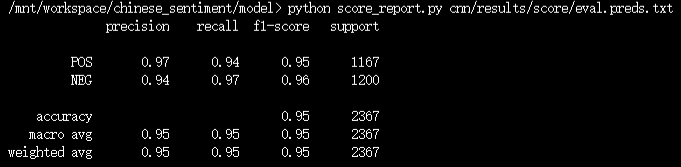
\includegraphics[width=0.9\linewidth]{sections//fig/cnn_res.png}
    \caption{CNN模型的训练结果}
    \label{fig:cnnres}
\end{figure}

最后,导出我们训练好的模型,进行自主输入测试。基于CNN的中文情感分析模型测试结果如图\ref{fig:cnn_test}。

\begin{figure}[H]
    \centering
    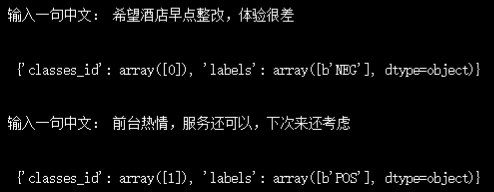
\includegraphics[width=0.9\linewidth]{sections//fig/cnn_test.png}
    \caption{CNN模型的测试结果}
    \label{fig:cnn_test}
\end{figure}

\subsection{基于BI-LSTM模型的中文情感预测}

首先,对分词后的语料样本进行Embedding,传入我们搭建好的BiLSTM模型中,进行模型训练。根据最后对模型输出的Logits进行Softmax操作,得到情感分析的结果的概率,与原标记比较。模型训练参数如表\ref{tab:bilstm_training_parameters}。

\begin{table}[H]
    \centering
    \begin{tabular}{c@{\hspace{40pt}}c}
        \toprule
        \textbf{Parameter} & \textbf{Value} \\
        \midrule
        dim & 300\\
        channel & 32\\
        dropout & 0.5\\
        num\_oov\_buckets & 1\\
        epochs & 25\\
        batch\_size & 20\\
        buffer & 3500\\
        \bottomrule
    \end{tabular}
    \caption{BiLSTM中文情感预测模型训练参数}
    \label{tab:bilstm_training_parameters}
\end{table}

进行多轮训练后,对训练好的模型进行评估。评价指标同基于CNN的中文情感分析模型(准确率、召回率与F1-score)。模型性能评估结果如图\ref{fig:bires}所示。

\begin{figure}[H]
    \centering
    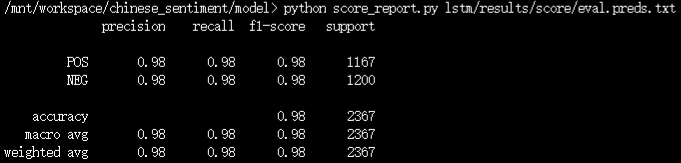
\includegraphics[width=0.9\linewidth]{sections//fig/bi_res.png}
    \caption{BI-LSTM模型的训练结果}
    \label{fig:bires}
\end{figure}

最后,导出我们训练好的模型,进行自主输入测试。基于BiLSTM的中文情感分析模型测试结果如图\ref{fig:bilstm_test}。

\begin{figure}[H]
    \centering
    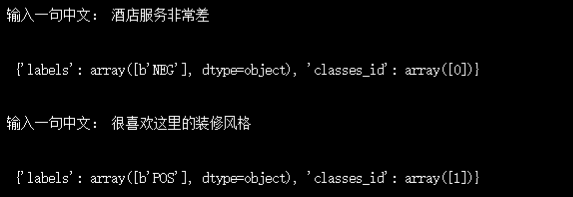
\includegraphics[width=0.9\linewidth]{sections//fig/bilstm_test.png}
    \caption{BiLSTM模型的测试结果}
    \label{fig:bilstm_test}
\end{figure}

\vspace{2em}

综上所述,我们分别采用CNN和BI-LSTM两种模型解决文本分类任务,并用于情感分析,达到不错的效果。 CNN模型在小数据集上训练,在验证集的准确率、号回率及F1因子均接近95\%。BI-LSTM模型,在验证集的准确率、号回率及F1因子均接近98\%。
\section{总结}

在本次实验中,我们探讨了基于CNN(卷积神经网络)和基于BI-LSTM(双向长短时记忆网络)的中文情感分析模型在处理文本情感分类任务中表现出色的情况。

CNN模型在中文情感分析中的表现优势:

\begin{itemize}
    \item \textbf{局部特征提取优势:}CNN模型能够有效地捕获句子中的局部特征和模式,有利于识别文本中的关键信息。
    \item \textbf{快速训练和预测: }由于CNN结构简单、参数相对较少,模型的训练速度较快,适用于快速迭代和实时预测场景。
    \item \textbf{适用于短文本情感分析: }在短文本的情感分类任务中,CNN模型展现出较好的效果,能够准确识别文本中的情感倾向。
\end{itemize}

BI-LSTM模型在中文情感分析中的表现优势:

\begin{itemize}
    \item \textbf{语义信息丰富:}Bi-LSTM模型能够捕获更丰富的语义信息和文本上下文关系,有助于更全面地理解文本情感。
    \item \textbf{长距离依赖:}通过双向信息流动,Bi-LSTM可以更好地处理长文本和长距离依赖关系,提高情感分析的准确性。
    \item \textbf{适用于深度文本理解:}对于对文本语境和更深层次的理解要求较高的任务,Bi-LSTM模型能够更好地解决这类问题。
\end{itemize}

综合来看,无论是CNN模型还是Bi-LSTM模型,在中文情感分析任务中都展现出不错的效果。CNN适用于简单且迅速的任务,而Bi-LSTM则更适合于需要深度文本理解和语境依赖的任务。根据具体场景和任务需求,选择合适的模型可以有效提升情感分析的准确性和效率。

\clearpage
\bibliographystyle{plain}
\bibliography{references}
%%%%%%%%%%%%%%%%%%%%%%%%%%%%%%
\label{LastPage}
\end{document}
\end